\documentclass[a4paper]{article}

\usepackage{INTERSPEECH2016}

\usepackage{graphicx}
\graphicspath{ {../} }
\usepackage{amssymb,amsmath,bm,bbm}
\usepackage{hyperref}
\usepackage{textcomp}
\usepackage{algorithm}
\usepackage{algpseudocode}
\usepackage{array}
\usepackage{multirow}
\usepackage[caption=false,font=footnotesize]{subfig}

\def\vec#1{\ensuremath{\bm{{#1}}}}
\def\mat#1{\vec{#1}}
\DeclareMathOperator{\round}{round}


\sloppy % better line breaks
\ninept

\title{Query Selection based on Latent Space Sampling}

%%%%%%%%%%%%%%%%%%%%%%%%%%%%%%%%%%%%%%%%%%%%%%%%%%%%%%%%%%%%%%%%%%%%%%%%%%
%% If multiple authors, uncomment and edit the lines shown below.       %%
%% Note that each line must be emphasized {\em } by itself.             %%
%% (by Stephen Martucci, author of spconf.sty).                         %%
%%%%%%%%%%%%%%%%%%%%%%%%%%%%%%%%%%%%%%%%%%%%%%%%%%%%%%%%%%%%%%%%%%%%%%%%%%
%\makeatletter
%\def\name#1{\gdef\@name{#1\\}}
%\makeatother
%\name{{\em Firstname1 Lastname1, Firstname2 Lastname2, Firstname3 Lastname3,}\\
%      {\em Firstname4 Lastname4, Firstname5 Lastname5, Firstname6 Lastname6,
%      Firstname7 Lastname7}}
%%%%%%%%%%%%%%% End of required multiple authors changes %%%%%%%%%%%%%%%%%

\makeatletter
\def\name#1{\gdef\@name{#1\\}}
\makeatother \name{{\em Benjamin Killeen}}

\address{University of Chicago \\
  {\small \tt killeen@uchicago.edu}
}

\begin{document}
\maketitle

\begin{abstract}
  The advent of deep learning has facilitated remarkable success on increasingly
  complex tasks. Large datasets are integral to this success, providing example
  labels which guide training, but many tasks are unrelated to existing
  datasets. In these cases, the choice of an \emph{initial query set} for
  annotation is crucial. A ``well-sampled'' query set can facilitate downstream
  approaches like semi-supervised or active learning, both of which require a
  small, labeled dataset. In this paper, we focus on sampling strategies using
  latent-space representations learned by auto-encoders, a self-supervised
  variant of deep neural networks. Furthermore, we constrain our latent-space to
  just two dimensions. Although potentially limiting, this focus allows for an
  easy visualization of latent spaces well-suited for initial exploration of the
  topic. We evaluate each sampling strategy using a simple classifier trained on
  just the initial query set.\footnote{Code and additional figures available at
    \href{https://github.com/bendkill/latens}{github.com/bendkill/latens}.}
\end{abstract}
\noindent{\bf Index Terms}: semi-supervised learning, active learning, computer
vision

\section{Introduction}
\label{sec:introduction}

% relevance of selecting a 
The collection and annotation of large datasets has been critical to the success
of deep learning. Wherever such data is available, it seems, the focus of the
community eventually results in a supervised learner with high performance, as
evaluated on the associated test set. Although that performance may extend to
examples from similar tasks, many application domains exist outside the scope of
established datasets. This is the case especially for scientific image analysis,
where the unique nature of each experiment sets it apart from conventional tasks
and obtaining labels can require significant investment, monetary- or
labor-wise, due to task complexity. Object detection, for instance, requires
more in-depth annotation than simple classification. In general, these scenarios
call for an approach that minimizes the labeling required to learn a specific
task, starting from scratch.

% discuss downstream approaches this is suitable for
Several sub-fields of machine learning confront this challenge. An active
learning approach, firstly, iteratively selects new examples for labeling in the
hopes of improving model performance at every step \cite{settles_active_2012}. A
popular sampling strategy incorporates the uncertainty of the model for each
unlabeled example \cite{settles_active_2012, lewis_sequential_1994}. Here, the
\emph{initial query set} is used to train the first iteration of the model,
before any active learning can take place. Typically, the initial query set is
selected randomly. This works well in many cases, but we hypothesize that a
well-sampled initial query set would result in a better initial model,
accelerating the active learning process. Although such tests are beyond the
scope of this paper, they remain an active area of inquiry. Secondly, a
semi-supervised approach, uses both labeled and unlabeled data during training
\cite{zhu_semi-supervised_2005}. Since the initial query set is actually the
\emph{only} query set, a well-sampled training set is of the utmost importance
for semi-supervised learning.

% define metric for success
At this point, the meaning of ``well-sampled'' is, admittedly, not readily
apparent. One would hope, for instance, that a well-sampled query set contains
instances from every class, in the case of classification, or from a wide range
of values, in the case of regression. Moreover, the representation of these
classes or values seemingly ought to be well-balanced, as if sampled
\emph{i.i.d.} not from the larger data, which may contain biases, but from the
natural distribution itself. However, these properties, however, are distinctly
qualitative. One way to quantitatively evaluate the quality of a sampling would
be through the performance of a downstream approach that uses an initial query
set, such as semi-supervised or active learning. In our experiments, we choose a
much simpler downstream approach, namely using the initial query set as the sole
training set for a simple classifier. The accuracy of this classifier, measured
on a withheld test set, serves as our measure for the ``well-sampled-ness'' of a
query set.

% narrow down to what this paper actually does (needs more work)
In this paper, we focus on sampling strategies that rely on a latent-space
representation of the unlabeled set. In particular, we use three types of
auto-encoders (AEs) to learn a two-dimensional representation of the unlabeled
set, which we sample according to distributions in the latent space
$\mathbb{R}^2$. There are many choices of distribution in the latent space; we
present four here that illustrate the properties of these representations.

\section{Method}
\label{sec:method}

\begin{figure}
  \centering
  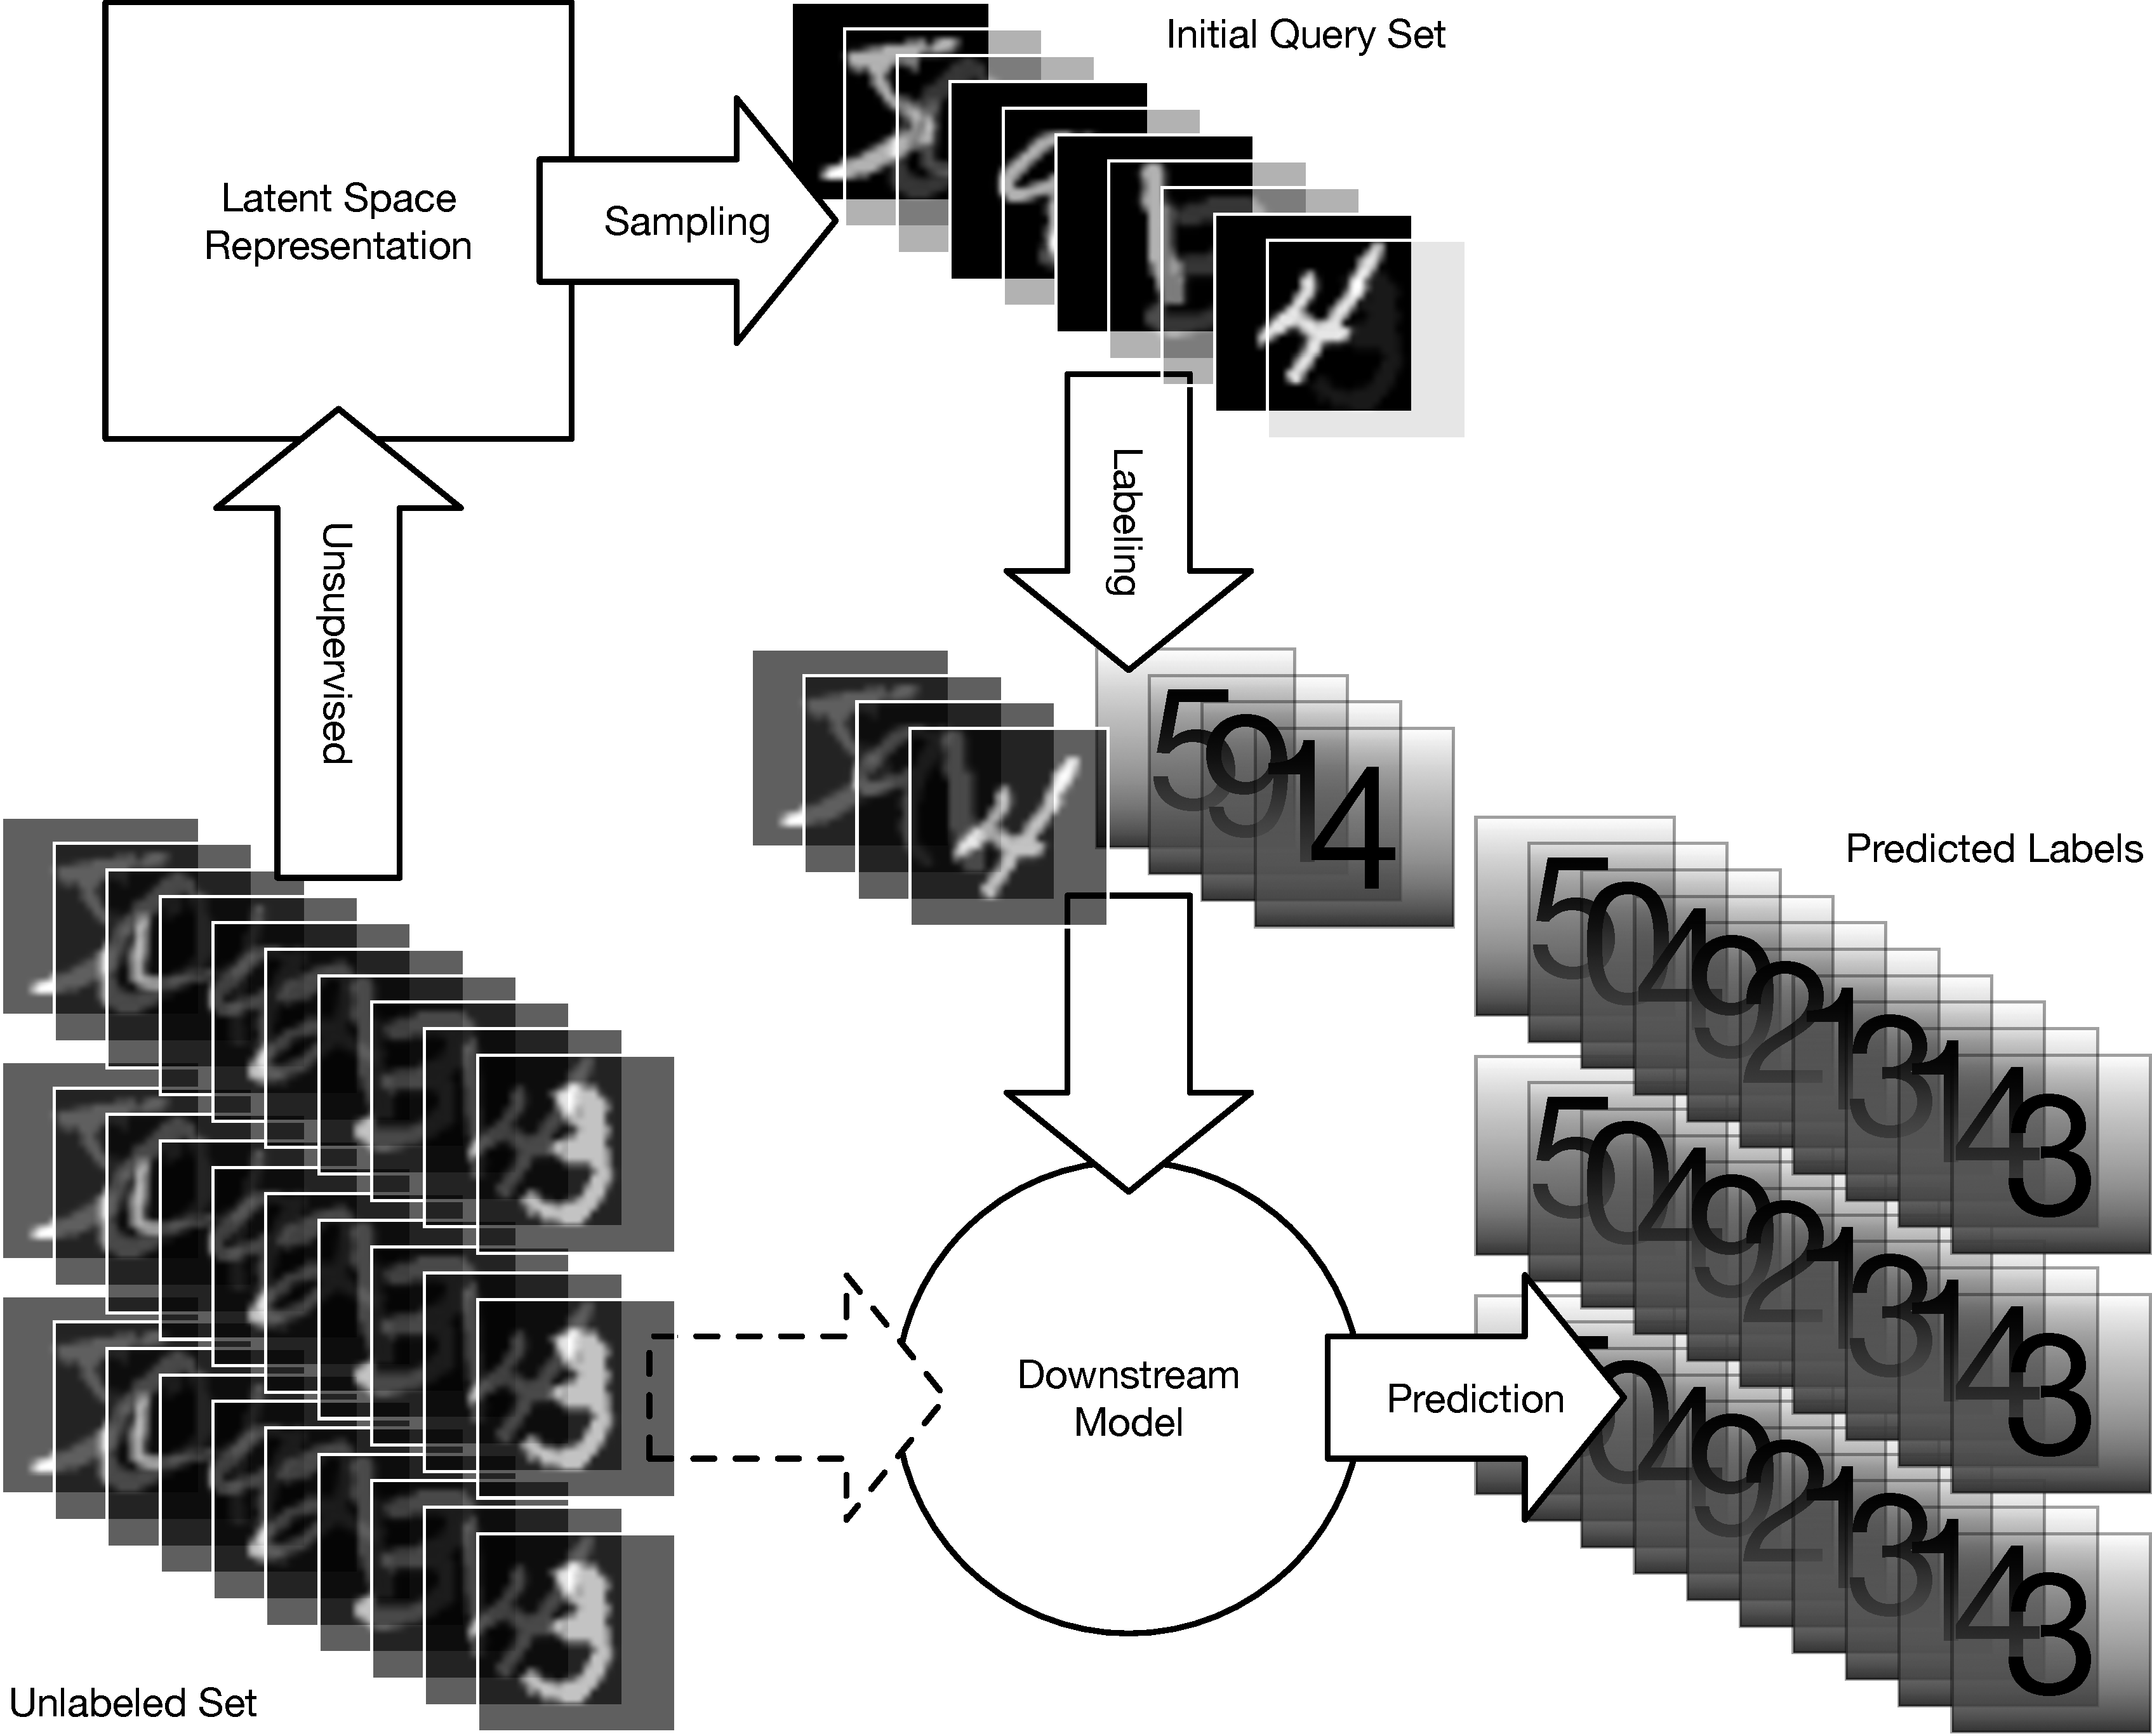
\includegraphics[width=\linewidth]{docs/query_selection}
  \caption{our initial query selection method (red) in relation to a downstream
    learning method (blue) like active or semi-supervised learning.}
  \label{fig:overview}
\end{figure}



Latent space sampling uses a large unlabeled dataset to identify examples which
should be labeled, according to one of several strategies (which we expound on
in this report). Initially, we consider data matrix
$X \in \mathbb{R}^{N\times D}$, where $N$ is the number of examples and $D$ is
the dimensionality of each example. In our experiments, we use
$28 \times 28 \times 1$ images, so $D = 784$. From this unlabeled set, we use an
auto-encoder to learn a low-dimensional or latent space representation
$Z \in \mathbb{R}^{N\times L}$ of $X$, where $L$ is the dimensionality of the
latent space.

Currently, we use a convolutional auto-encoder (CAE) to learn a 10-dimensional
encoding of the dataset \cite{krizhevsky_imagenet_2012,
  goodfellow_deep_nodate}. The CAE consists of an encoder and a decoder. The
encoder uses multiple $3\times 3$ convolutional layers broken up with two
$2\times 2$ max-pooling to reduce the image dimensions to $7\times 7 \times 64$
in the last convolutional layer. This is followed by two dense layers with 1024
and $L$ nodes respectively. The decoder reverses this architecture, replacing
max-pool layers with $2\times 2$ transpose convolutions. In each layer, we use
the ReLU activation function, except for the encoder's final layer, the
``representation layer.'' The choice of activation for the representation layer
is driven by a combination of performance considerations---what generates good
encodings---as well as sampling considerations. Initially, we envisioned that
constraining the latent space to the hypercube $[0,1]^L$ would result in an
easily sampled representation with good spread.\footnote{This vision has since
  changed. See Section~\ref{sec:discussion} for details.} Experiments with the
sigmoid activation function proved unsatisfying, and so following Nair and
Hinton's Rectified Linear Unit \cite{nair_rectified_nodate}, we employ a clipped
linear unit (CLU) given by $f(x) = \min(1, \max(0,x))$, in our initial
experiments. This choice was made in order to guarantee a hypercube constrained
representation $Z \in [0,1]^{N\times L}$ while still providing the performance
advantages of the ReLU.

Once we obtain $Z$, we select a sampling or index set $Q \subseteq [N]$ based on
the distribution of $Z$. One strategy, which we employ in our preliminary
experiments, is to sample from this space according to a random uniform
distribution. As described in Algorithm~\ref{alg:uniform-sampling}, we draw a
point $z \in [0,1]^L$ uniformly and, if any data-point representation $z_i$
exists within a given distance $d(z,z_i)$, then we add $i$ to the query
set. Figure~\ref{fig:overview} provides an overview of this representation
learning and sampling process.

\begin{algorithm}
  \begin{algorithmic}[1]
    \Require \hfill %
    \begin{itemize}
    \item the encoding $Z \in \mathbb{R}^L$,
    \item clustering $\mathbf{S} = \{S_1 , \dots, S_C\}$ on $Z$,
    \item distributions
      $\{f_S : \mathbb{R}^L \rightarrow \mathbb{R}| S \in \mathbf{S}\}$, and
    \item distance threshold
      $t \in \mathbb{R}$, $n \in \mathbb{N}$.
    \end{itemize}

    \State $Q \gets \{\}$ %
    \For {Cluster $S \in \textbf{S}$} %
    % \State Determine distribution $f : \mathbb{R}^L \rightarrow \mathbb{R}$
    % based on cluster points $\{z_i | i \in S\}$. %
    \State $n_S \gets \round\left(n \frac{|S|}{N}\right) $ %
    \State $Q_S \gets \{\} $ %
    \While {$|Q_S| < n_S$} %
    \State Draw $z \sim f_S$ %
    \For {$i \in S$} \Comment the $i$th row of $Z$, in cluster $S$ %
    \If {$||z - z_i||_2 < t$} %
    \State $Q_S \gets Q_S \cup \{i\}$ %
    \EndIf %
    \EndFor %
    \EndWhile %
    \State $Q \gets Q \cup Q_S$ %
    \EndFor %
    \State \Return $Q$ %
  \end{algorithmic}
  \caption{Select examples from the clustered encoding $Z$ according to a
    distribution $f_S$ on each cluster $S$. Applies to sampling strategies
    without clustering if $\mathbf{S} = \{[N]\}$.}
  \label{alg:sampling}
\end{algorithm}

\section{Results}
\label{sec:results}

\begin{figure}
  \centering
  \subfloat[]{
    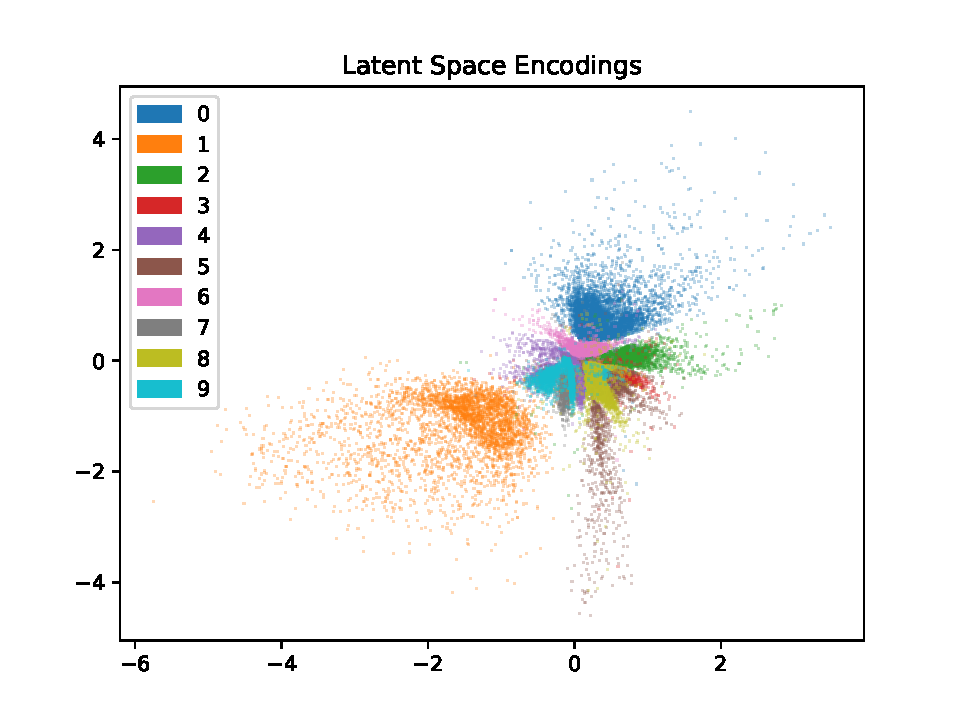
\includegraphics[width=\linewidth]
    {models/unbalanced_mnist_vae_e300_L2_b64/encodings}
    \label{fig:vae-encodings}
  } \\
  \subfloat[]{
    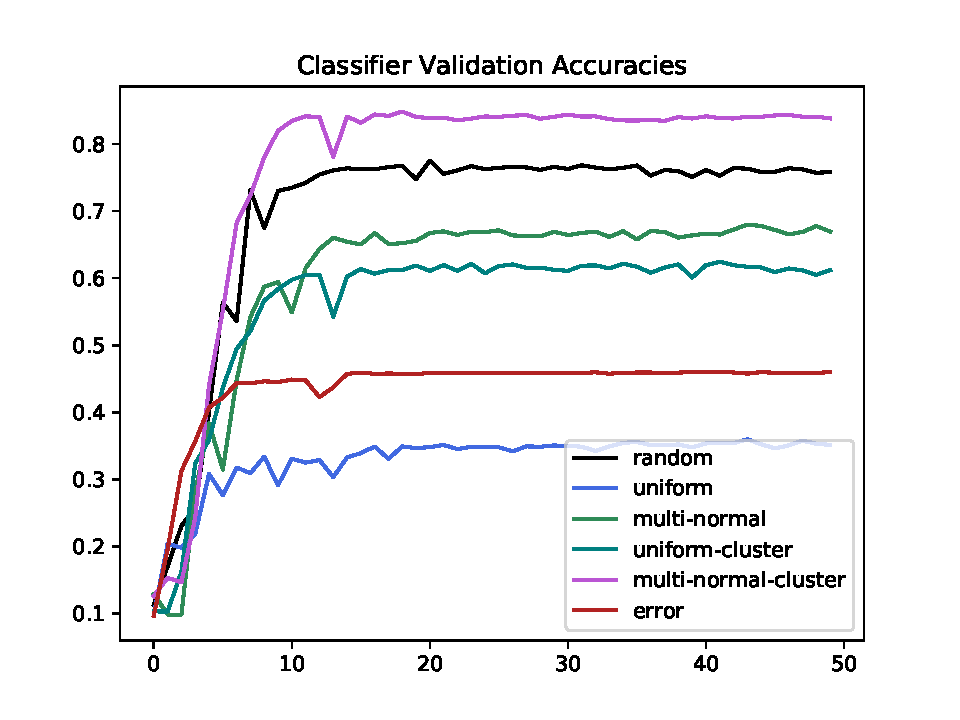
\includegraphics[width=\linewidth]
    {models/unbalanced_mnist_vae_e300_L2_b64/classifier_val_accs_100}
    \label{fig:classifier-losses}
  }
  \caption{Latent-space encoding for the MNIST training set using a VAE.}
  \label{fig:unbalanced-mnist-results}
\end{figure}

\begin{table*}[]
  \centering
  \begin{tabular}{|l|l|m{3em} m{3em}|m{3em} m{3em}|}
    \hline
    \multicolumn{1}{|c|}{AE Type} & \multicolumn{1}{|c|}{Sampling Strategy}
    & \multicolumn{2}{|c|}{Balanced MNIST} & \multicolumn{2}{|c|}{Unbalanced MNIST} \\
    & & \multicolumn{1}{|c}{1000} & \multicolumn{1}{c|}{100} & \multicolumn{1}{|c}{1000} & \multicolumn{1}{c|}{100} \\
    \hline
    --- & Random & $94.0_{\pm .2}$ & $80.9_{\pm 1.8}$ & $92.6_{\pm .4}$ & $76.6_{\pm .6}$\\
    \hline
    --- & AE-error & $93.8_{\pm .3}$ & $76.6_{\pm .4}$ & $57.8_{\pm .2}$ & $46.4_{\pm .2}$ \\
    \hline
    \multirow{4}{4em}{Conv}
    & Uniform
      & 72.7 & 38.1 & 62.9 & 44.6 \\
    & Normal
      & 93.1 & 70.3 & 90.5 & 66.3 \\
    & Clustered Uniform
      & 89.6 & 71.6 & 89.2 & 71.5 \\
    & Clustered Normal
      & 94.4 & 80.9 & 92.8 & 79.6 \\
    \hline
    \multirow{4}{4em}{VAE}
    & Uniform
      & 68.2 & 38.8 & 62.4 & 35.3 \\
    & Normal
      & 92.1 & 69.9 & 91.7 & 66.5 \\
    & Clustered Uniform
      & 86.1 & 67.3 & 86.8 & 62.1 \\
    & Clustered Normal
      & 94.3 & \textbf{82.9} & 92.3 & \textbf{85.0} \\
    \hline
    \multirow{4}{4em}{t-SNE Style}
    & Uniform
      & 69.3 & 56.6 & 85.7 & 53.0 \\
    & Normal
      & 93.6 & 82.3 & 91.7 & 77.0 \\
    & Clustered Uniform
      & 87.3 & 71.6 & 91.6 & 76.6 \\
    & Clustered Normal
      & 94.4 & 78.9 & 92.4 & 75.9 \\
    \hline
  \end{tabular}
  \caption{Test-set accuracies (\%) for a classifier trained on sample sets from
    both the balanced and unbalanced MNIST data. As can be seen, the advantage
    of latent space sampling is most apparent when the original data is
    unbalanced and the sample size is small enough to reflect it.}
  \label{tab:results}
\end{table*}

\section{Discussion}
\label{sec:discussion}

\section{Conclusions}
\label{sec:conclusion}

\section{Acknowledgements}
\label{sec:acknowledgements}

Thanks to Gordon Kindlmann for computational resources. Implementation and
sampling strategies original work, as well as t-SNE Style autoencoder.

\newpage
\eightpt
\bibliographystyle{IEEEtran}

\bibliography{report}

\end{document}

%%% Local Variables:
%%% mode: latex
%%% TeX-master: t
%%% End:
